% ******************************* Thesis Appendix B ********************************
\chapter{} 
\label{app:missionplan}

\graphicspath{{Appendix2/Figs/}}


\renewcommand{\thefigure}{B\arabic{figure}}

\setcounter{figure}{0}

The following image is a screenshot of an example mission plan, where each row of text is one MAVLink message. When created in one of the mission planning software products, the non-integer values are given to 6 decimal places. Where new messages have been inserted, decimal places have not been included apart from where necessary. The 4th entry in each row is the mission command ID; 178 commands are commanding the UAV to fly at a certain speed, whilst the 85, 86, and 87 are Dubins left, right, and straight commands respectively. For the new Dubins turn commands, the 5th entry is the duration to fly that segment of the path, given in milliseconds. Please note that the waypoint numbering is not incremented properly, although this is unimportant as it has no effect on either ArduPlane or the simulator.

\begin{sidewaysfigure}[htbp!] 
\centering    
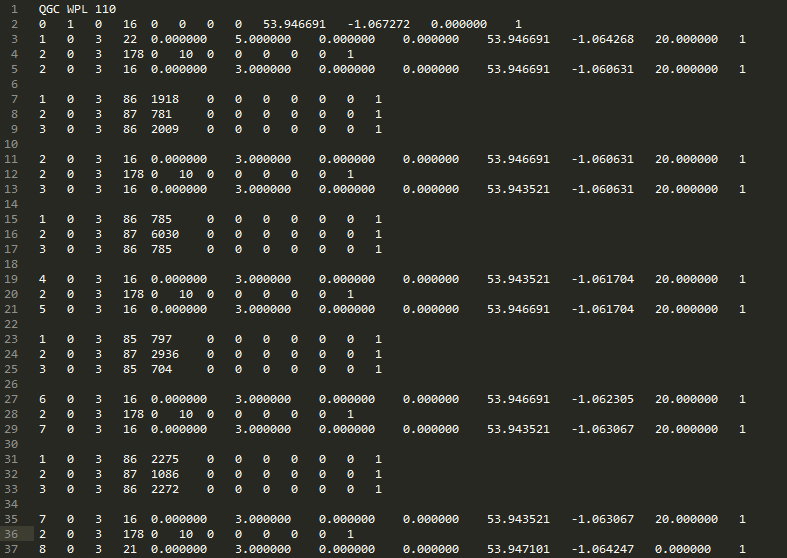
\includegraphics[width=0.8\textwidth]{MissionPlan}
\caption{A full mission plan displaying the format of a MAVLink message and the new Dubins turn commands inserted between waypoints}

\end{sidewaysfigure}